\label{ch:experimental_techniques}

\section{Grinding of Glass}
\label{sec:grinding_glass}

The manufacturing process of polished glass pieces typically begins with grinding, which, thanks to its ability to achieve surface flatness while maintaining high MRRs on hard and brittle materials, is considered one of the most important and feasible machining technologies. However, grinding can induce surface and subsurface damage on the glass sample. Consequently, chemical mechanical polishing (CMP) is employed to eliminate these residual defects [CMP of glass disk].
\\
Grinding too is a complex process, especially when applied to glass due to the nature of the material. The most used abrasive materials are silicon carbide or diamond grinding wheels [Grinding of Glass: the mechanics of the process *(GoG)*]. 
\\
Previous research shows that both permanent viscous flow and brittle fracture can occur during the grinding of glass surfaces. 
Viscous flow is the main grinding mechanism when using silicon carbide. On the contrary, when using diamond grinding wheels, glass is grinded mostly through brittle fracture of particles from the surface.

\subsection{Non-Newtonian Flow of Glass Particles}
It is widely recognized that glass can be made to flow without fracturing under significant hydrostatic compressive stresses, even at ambient temperature [GoG]; this can happen because the local surface temperature in the grinding zone can easily exceeds the glass's softening point. The pressure conditions, favorable for the flow of glass, are also expected to exist at the cutting edge of an abrasive grain during grinding.
\\
It has also been observed that most of the grinding energy is dissipated in the material by viscous deformation [GoG]. For this reason, glasses with high softening temperatures also have a high specific grinding energy, that is defined as the proportionality constant between the work expended in the process and the rate of material removal.
\\
Additionally, it has been observed that there is a correlation between the increase in specific grinding energy and the decrease in particle grain sizes [GoG].
\\
Numerous experimental investigations have clearly demonstrated that when soda-lime glass is subjected to sufficiently high axial stress or pressure, it exhibits a nonlinear mechanical response, and an irreversible deformation takes place, a phenomenon known as inelasticity or material nonlinearity [Material Nonlinearity and Inelasticity] [non-Newtonian viscous flow]. Studies of the viscosity of stable soda-lime glass under high shear stress have revealed a non-Newtonian viscosity of the pseudoplastic type. In this behavior, if the applied stress rate exceeds a certain threshold value, catastrophic failure of the material occurs, leading to the formation of numerous cracks and an eventual brittle fracture of the glass sample [Non-Newtonian Viscous Flow].
\\
The interpretation of this non-Newtonian behavior is attributed to atomic structural rearrangements within the glass material. These rearrangements play a significant role in determining the material's mechanical response under high stress conditions, ultimately influencing its flow and fracture characteristics during the grinding process.
\section{Chemical Mechanical Polishing}
\label{sec:CMP}
Chemical mechanical polishing (CMP) has been a widely used planarization method in various industries, including integrated circuits manufacturing and glass surface polishing, for many decades. The effectiveness of CMP in achieving planar, smooth, and damage-free surfaces is influenced by numerous factors related to the sample carrier structure, polishing pad, slurry composition, and other process parameters. Since both chemical and mechanical actions play a role in CMP, and since they are influenced by multiple variables, understanding the complexity of the CMP mechanism is still a great challenge and is an actively researched topic.
\\
CMP aims to produce planar surfaces on target materials by removing micro and nano-sized particles, sometimes acting even on the atomic-scale; with the goal of achieving sub-nanometer level roughness while minimizing surface and subsurface damage [CMPTE]. The surface smoothing effect observed in CMP is attributed to various mechanisms, including the non-Newtonian flow of glass material, fretting and mechanical abrasion caused by friction between the glass and the polishing tool, and chemical reactions leading to surface decomposition.
\\
In general, mechanical abrasion and chemical removal are typically the predominant mechanisms, leading to the use of the term: "chemo-mechanical polishing" [Gerhard et al. Appl Surf Sci].
\\
Mechanical removal is mostly based on the interaction of the glass surface with abrasive grains, such as cerium oxide or aluminum oxide, present in an aqueous polishing slurry. On the other hand, chemical removal involves complex processes such as diffusion of water molecules into the glass sample, redeposition of silica on the surface during polishing, and diffusion of polishing agents into the surface of the glass [Cook, 1990].
\\
Polishing is not only needed to obtain a transparent surface of an optical glass component with the required accuracy, but also to remove digs, pits, and microcracks induced by the previous processes to obtain smooth surfaces that minimize scattering [Optics Manufacturing (Gerhard)].

\subsection{CMP Technique}
\label{subsec:cmp_technique}

Chemical mechanical polishing (CMP) is a process that, by definition, combines chemical and mechanical actions to enhance the material removal rate (MRR), which quantifies the amount of material removed per unit time. The MRR is influenced by various factors including the system configuration, the properties of the abrasive pad, and the composition of the polishing suspension employed.
\\
Depending on the layout of the polishing machine, different approaches and principles can be applied for polishing.
\\
There are four main types of commercially available CMP equipment commonly used in industry, as shown in Figure~\ref{fig:cmp_equipment}: 
\begin{figure}[H]
    \centering
    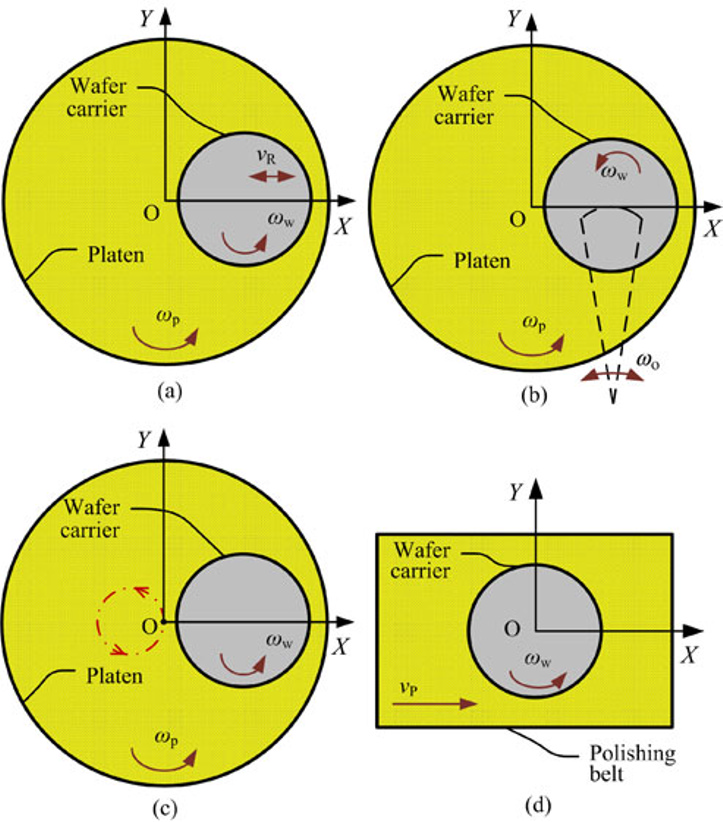
\includegraphics[width = 0.4\textwidth]{chapter_2/cmp_equipment.png}
    \caption[Schematic of different types of CMP equipment.]{ Schematic of different types of CMP equipment: (a) rotary type, reciprocation mode, (b) rotary type, oscillation mode, (c) orbital type, and (d) linear type.}
    \label{fig:cmp_equipment}
\end{figure}
[taken from CMP theory and experiments]

\begin{enumerate}
    \item Rotary type polisher with a sample carrier featuring a reciprocating motion along the platen diameter.
    \item Rotary type polisher with a sample carrier exhibiting an oscillatory motion.
    \item Orbital type polisher with the platen having an orbital rotation.
    \item Linear type polisher equipped with a linear motion belt as the polishing pad.
\end{enumerate}
The movement of the carrier and the platen generates the necessary relative motion for the polishing process, while a slurry, containing particles and chemical solutions, is delivered onto the pad to act as the abrasive [CMPTE]. Through the combined chemical actions of the solutions and the mechanical actions of the particles, micro material removal occurs, enabling surface polishing and finishing to be realized.
\\
The MRR, non-uniformity, and surface quality are key indicators of machining and CMP process efficiency. These parameters are influenced by some major factors such as the system configuration, process variables (e.g., down pressing force of the sample on the pad, relative velocity of the pad), and consumables (e.g., slurry concentration). The synergetic interaction of these input variables determines the final polishing results by affecting the sample-pad interaction and material removal process. 

\subsection{Modeling of CMP}
The removal rate in CMP is determined by several parameters at the sample-pad interface, including pressure, temperature, and slurry distribution over the active surface. Many process variables, such as sample pressing downforce, pad rotation speed, slurry characteristics and the employed pad material, can influence the final polishing outcomes [CMPTE].
\\
A theoretical description of the polishing of optical glasses is thus a complex task since such polishing processes are based on different interacting mechanisms. These different mechanisms have been described by some models: the removal, the flow, the chemical, and the fretting hypothesis [Optics Manufacturing (Gerhard)].
\\
Under the removal hypothesis, the sharp edges of the abrasive particle grains of the polishing agent enter in contact with the surface of the glass digging out small particles. Since these interactions preferentially target the roughness peaks of the working surface, a smoothing effect is obtained over time [Optics Manufacturing (Gerhard)].
\\
The flow hypothesis says that in addition to the mechanical removal by abrasion, the polishing agent grains also perform an irreversible displacement of the glass material. Here, due to the friction between the work piece surface and the polishing pad and grain, the local temperature can rise above the softening point of the glass and as a result, roughness peaks are dislocated into roughness valleys or digs by material flow. 
\begin{figure}[H]
    \centering
    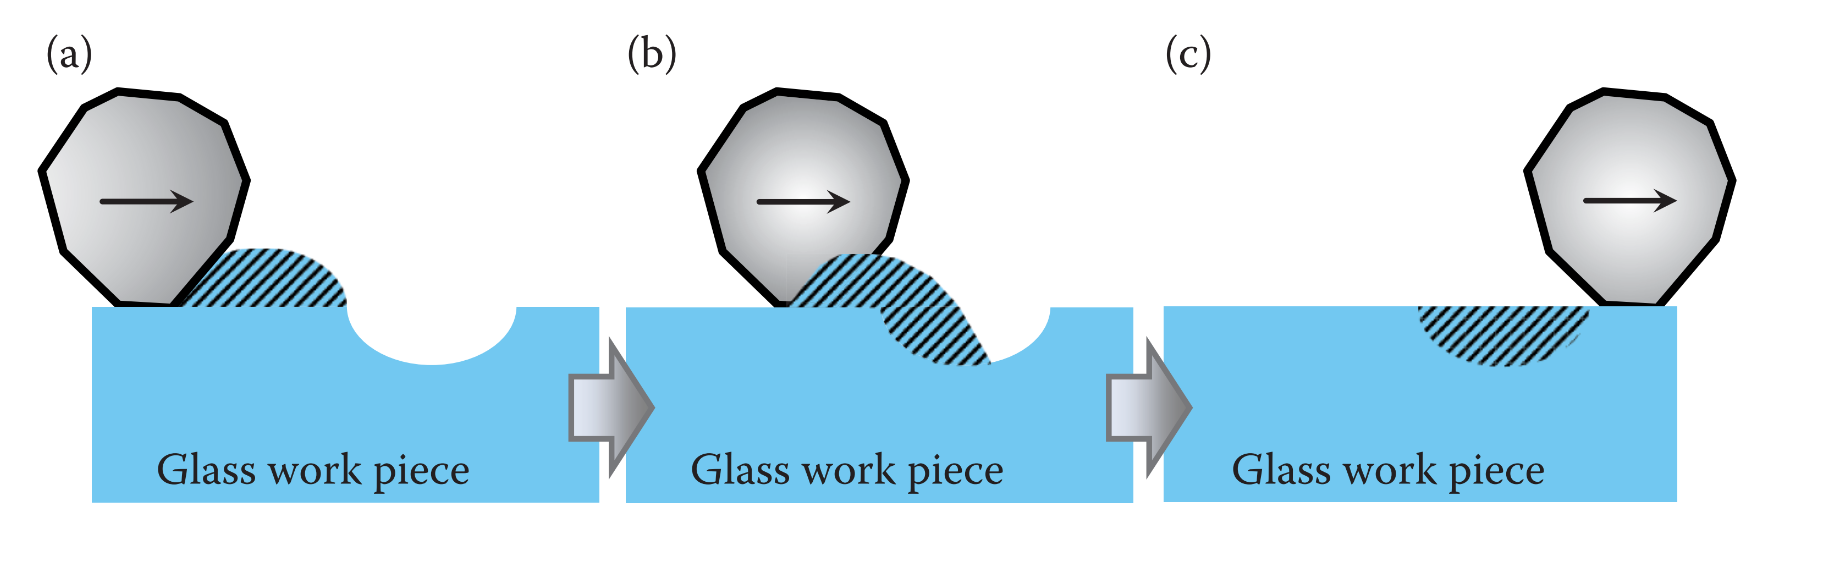
\includegraphics[width = \textwidth]{chapter_2/flow_hypothesis.png}
    \caption[Visualization of the flow hypothesis.]{ Visualization of the flow hypothesis; roughness peaks (dashed structure) are softened by wear in the course of the polishing process (a) and dislocated into roughness valleys or digs (b), consequently resulting in a leveling of the surface (c).}
    \label{fig:flow_hypothesis}
\end{figure}
[image taken from optics manufacturing Gerhard]
Under the chemical hypothesis are described the chemical reactions that take place on the surface of the target glass sample. Such reactions are supported by hydrolytic scission of bonds of the glass network [Optics Manufacturing (Gerhard)] according to Equation~\ref{eq:hydrolytic_scission}:
\begin{align}
\ce{(SiO2)_x + 2H2O <-> (SiO2)_{x-1} + Si(OH)4} \label{eq:hydrolytic_scission}
\end{align}
The rate of the reaction is controlled by the diffusion of water molecules at the surface of the glass [Cook, 1990]. The depth of this diffusion layer can be estimated, after a given time “$t$”, by the relation: 
\begin{align}
    d_{dif}\ \approx\ 2\sqrt{Dt} \label{eq:diff_length}
\end{align}
Where D is the diffusion coefficient of water into glass and its value can range from $10^{-15} \:cm^2/s$ to $10^{-18}\: cm^2/s$ : (Nogami and Tomozawa, 1984; Lanford et al., 1985).
\\
As a result of this phenomenon, hydrated silica is deposited on the sample surface during polishing, consequently leading to the formation of a silica gel layer [Optics Manufacturing (Gerhard) (Iler, 1979; Cumbo and Jacobs, 1994)] that contributes to surface smoothing, since it can accumulate in digs and scratches filling those geometric surface defects. 
\\
The last studied mechanism is based on the material removal due to fretting, arising from the synergy between two physical factors: the contact pressure of the polishing tool on the glass surface and their relative movement [Optics Manufacturing (Gerhard) (Dimatteo, 1997)]. This early model, developed by Frank W. Preston in the late 1920 (Preston, 1927) describes the MRR through an empirical equation as follows:
Formula (8.4) in [Optics Manufacturing (Gerhard)] and [CMPTE]
\begin{align}
    MRR=kPV \label{eq:material_removal}
\end{align}
Here, “$k$” is an empirical constant determined from experimental data, P is the pressure applied to the sample and $V$ is the relative velocity between the glass and the polishing tool.
\\
This equation only considers the mechanical contributions to the MRR, neglecting the chemical actions. In this way, the polishing process can be described as a simple two body wear problem, where the target sample is pressed down on a polishing pad and moving at a fixed speed.
\\
To increase the accordance with experimental data, an alternative expression for the Preston equation have been proposed: $MRR=kP^\alpha V^\beta$[CMPTE]; where the dependence of the $MRR$ relative to the pressure and velocity is no longer linear. However, this model still fails to correctly describe processes where chemical interactions are crucial.

\section{Polishing Elements}
\label{sec:polishing_elements}
In the polishing process a resilient pad, a target sample to be polished, and an abrasive slurry are the key components. The process involves pressing a glass sample face down onto a rotating polishing pad while a slurry containing abrasive particles and chemical additives flows between them. This mechanical and chemical action removes material from the sample, resulting in a smoother surface.
\subsection{Polishing Pad}
Different types of pads can be utilized for polishing, even though traditionally the typical polishing pad was made of pitch [Optics Manufacturing (Gerhard)], a natural viscoelastic polymer, also known as bitumen or asphalt, derived from petroleum or tar. Today polishing pads are typically made of porous polyurethane [CMPTE] with additional components added to tune the pad hardness [CMPTE 4]. This material is capable of higher process velocities, and it is less sensitive to temperature changes [Optics Manufacturing (Gerhard)]. 
\\
The hardness of the pad is a critical property that can influence both the material removal rate (MRR) and the uniformity of polishing [CMPTE]. Different applications and types of target materials may require either hard or soft pads.
\\
Both the bulk of the pad and the surface are full of micropores, which are useful for retaining the abrasive particles of the slurry; these micropores play a crucial role in the polishing process by facilitating the interaction between the pad, the slurry, and the sample. As shown in Figure~\ref{fig:hard_soft_pad}
\begin{figure}[H]
    \centering
    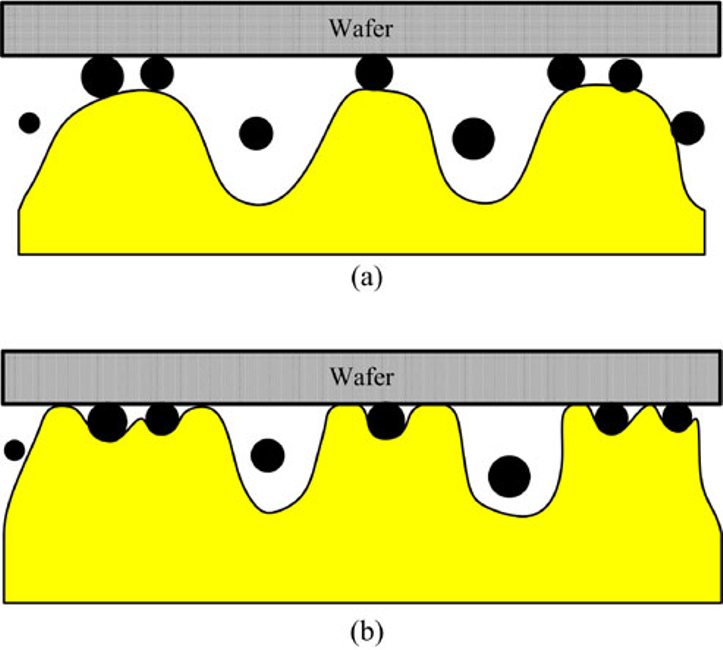
\includegraphics[width = 0.6\textwidth]{chapter_2/hard_soft_pad.png}
    \caption[Comparison between a hard pad and a soft pad.]{ Contact status of (a) hard pad, and (b) soft pad. }
    \label{fig:hard_soft_pad}
\end{figure}
During CMP, the physical properties of the pad, such as hardness and surface roughness, are expected to change due to mechanical loads and chemical reactions occurring during the polishing. These changes could significantly impact the process, so they should be limited to ensure consistent results.

\subsection{Polishing Suspension (Slurry)}
\label{subsec:polishing_slurry}

The slurry used in CMP is a complex mixture consisting of abrasive materials dispersed in water along with various chemicals, including oxidants, inhibitors, and bases to adjust the pH. Abrasive particles such as \ce{SiO2}, \ce{CeO2}, and \ce{Al2O3}, with sizes ranging from 10 nanometers to some micrometers [Optics Manufacturing (Gerhard)], are commonly used in industrial CMP processes. The mass concentration of the polishing agent relative to the total slurry usually spans from 5\% to 30\% [Bliedtner and Gräfe, 2008].
\\
The choice of a particular polishing agent depends on the material of the work piece [Optics Manufacturing (Gerhard)], while the properties of the abrasive particles, such as the size distribution, chemical composition, and concentration, as well as the pH of the slurry, will have a significant impact on the material removal rate ($MRR$), uniformity, and surface quality of the polished material [CMPTE]. For example, at pH values of 3.0 and 10.0, the material removal is primarily driven by chemical corrosion, while at a pH around 7.0, the mechanical action of abrasive particles becomes the dominant factor contributing to the $MRR$. [Effects of chemical additives of CMP]
\\
During CMP, the slurry plays a crucial role at the interface between the wafer and the polishing pad. The flow of slurry brings abrasive particles and chemicals to the interface, where they initiate the polishing process by removal or material flow [Optics Manufacturing (Gerhard)]. The slurry will form a lubricating film, reducing friction forces between the wafer and pad, and the fluid presence can also help support some of the downforce, thereby relieving pressure from the pad [CMPTE].
\\
Physical models have shown that in slurry with a size distribution of abrasive particles, only the larger particles make direct contact with the pad and the sample, leading to effective material removal [Effect of chemicals on CMP of glass substrates]. 

\section{Side Effects of Polishing}
\label{sec:polishing_side_eff}

The uniformity of glass substrate surfaces in terms of index of refraction, chemical composition, and roughness is crucial in many different applications. However, during the manufacturing process, from rough grinding to fine polishing, nonuniform surfaces can arise. This is due, for example, to the presence of contaminants inside the glass, caused by residues of operating materials used during manufacturing as, most commonly, polishing agents.
\\
One significant chemical mechanism, happening on the surface of the sample during CMP, is the formation of a silica gel layer, also known as the redeposition layer [Gerhard et al appl opt 2017].
\\
This layer forms as water penetrates the glass surface, leading to hydrolytic scission of the glass network, which results in the formation of a thin layer consisting of hydrated silica, or silanol. During the growth of this layer on the surface, also known as Beilby layer, residues from polishing agents and other elements from the polishing suspension can remain embedded within it [Gerhard et al appl surf sci].
\\
For example, some studies [Kozlowski] have shown that aluminum from corundum-based abrasives can exceed a mass fraction of 1000 ppm on the glass surface. This retention occurs as particles from the polishing slurry accumulate within surface defects such as digs, scratches, and microcracks formed during earlier manufacturing steps [Gerhard et al Appl Opt 2017].

\begin{figure}[H]
    \centering
    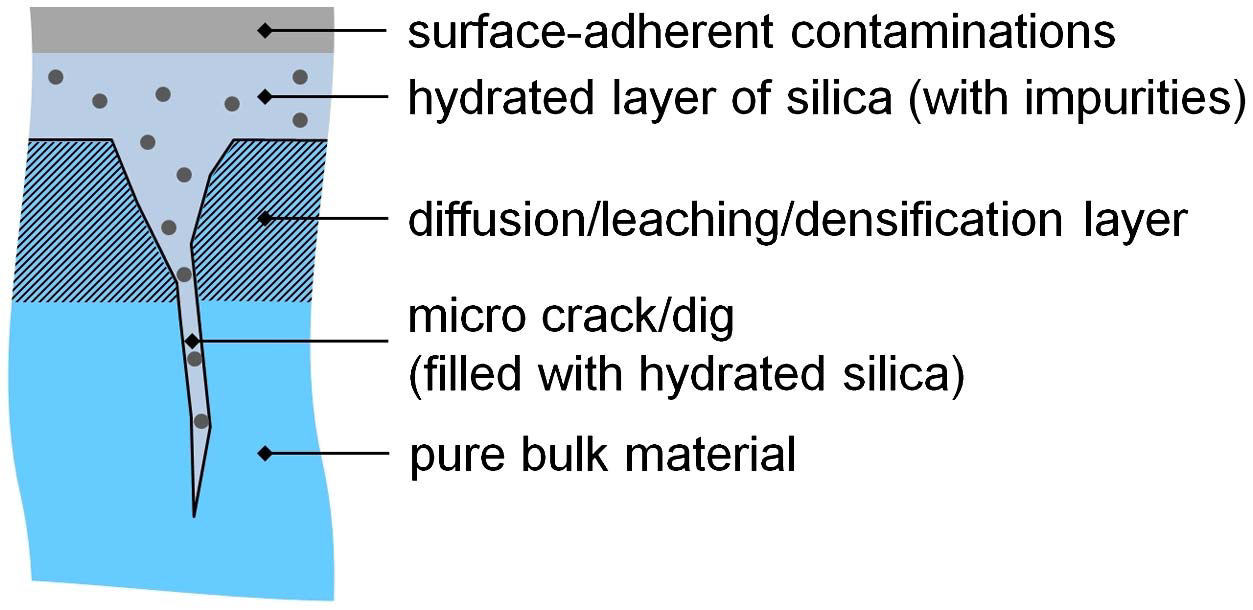
\includegraphics[width = 0.6\textwidth]{chapter_2/micro_cracks.png}
    \caption[Schematic of a surface defect generated during optics manufacturing.]{ Schematic presentation of a typical surface defect generated
during classical manufacturing of optical surfaces. }
    \label{fig:micro_cracks}
\end{figure}
[taken by Gerhard app optics]
\\
As a result of these processes, visually clean polished glass surfaces can exhibit significant optically active contaminations [Gerhard et al Appl Opt 2017]. These contaminations may include surface adherent contaminants such as hydrocarbonaceous compounds and residues from polishing agents. The remaining silica gel layer and contaminants on the surface can also lead to negative effects such an increase in near-surface absorption consequently lowering the laser-induced damage threshold [Optics Manufacturing (Gerhard)].

\section{Diffusion}
\label{subsec:diff}

As already mentioned in Chapter~\ref{sec:CMP}, diffusion is a core process in optics manufacturing; following is a brief exposition on the main characteristics of the mechanism.
\\
Diffusion is a physical and time dependent mechanism that drives the flow of particles from a low concentration portion of a medium to a high concentration one. The process is purely thermodynamical, the difference between the chemical potential, i.e. the potential associated with the concentration of particles, causes a difference between the Gibbs free energy of the two areas and leads to the flow of material in order to achieve equilibrium.
\begin{figure}[H]
    \centering
    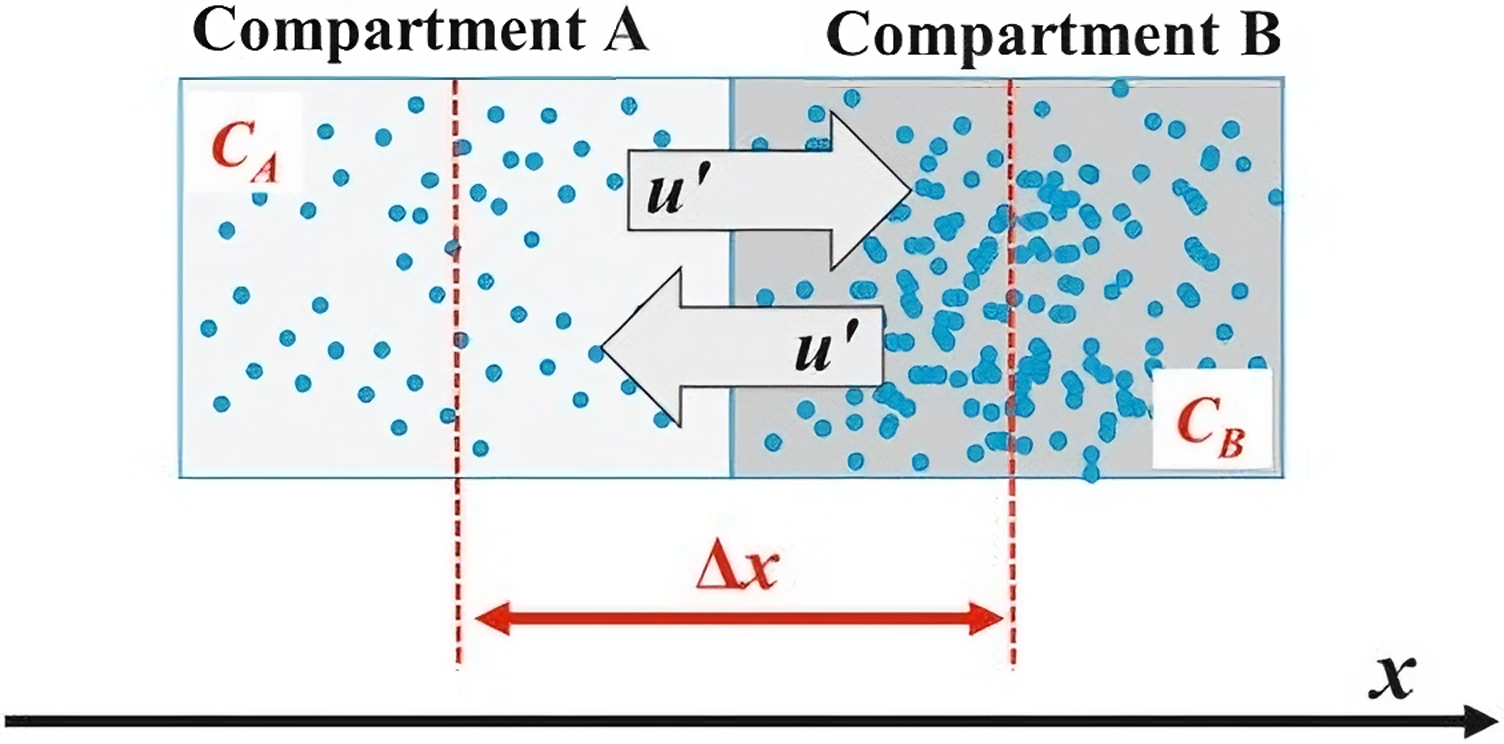
\includegraphics[width = 0.5\textwidth]{chapter_2/diffiusion_upscaled.jpg}
    \caption[]{Diffusion driven by the difference in concentration in the two compartments.}
    \label{fig:diff_drawing}
\end{figure}
[taken by https://www.sciencedirect.com/topics/earth-and-planetary-sciences/molecular-diffusion]
The simplest diffusion processes are called “normal” (or “Fickian”) and can be modelled by the two Ficks’s laws. 
\\
The first one is:
\begin{align}
    \vec{J}=-D\vec{\nabla}C \label{eq:first_law_3d}
\end{align}
Where the vectorial flow of particle $\vec{J}$ is proportional to the gradient of the concentration with a proportionality constant “$D$”, which is called diffusion coefficient. This coefficient, in general, will depend on both the substrate and the species diffusing into it, as well as on other external parameters like temperature and pressure. 
\\
It is very common to model diffusion processes one dimensionally, the first Fick’s law then becomes:
\begin{align}
    J=-D\frac{\partial C}{\partial x} \label{eq:first_law_1d}
\end{align}
Where we can clearly see that without any difference in concentration along x there is no flow of particles.
\\
The first law only describes the spatial dependence of the process. To also introduce the time dependency, it is necessary to also consider the second Fick’s Law, which states:
\begin{align}
   \frac{\partial C}{\partial t}=D\nabla^2C \label{eq:second_law_3d}
\end{align}
Under a 1-D approximation Equation~\ref{eq:second_law_3d} becomes:
\begin{align}
   \frac{\partial C}{\partial t}=D\frac{\partial^2C}{\partial x^2} \label{eq:second_law_1d}
\end{align}
Where the same proportionality constant D relates the concentration derivative with respect to time to its second spatial derivative.
\\
This partial differential equation can be solved by taking as boundary condition a fixed concentration $C_0$ at a certain value of $x$ (usually $x = 0$). This models a situation where a constant source of external diffusant is applied at one of the surfaces of a material.
\\
The solution of the equation, which is only valid for positive values of $x$, is:
\begin{align}
    C\left(x,t\right)=C_0\operatorname{erfc}\left(\frac{x}{2\sqrt{Dt}}\right) \label{eq:fick_solution}
\end{align}
Where $\mathrm{erfc}$ is the complementary of the error function and is defined as:
\begin{align}
   \operatorname{erfc}z=1-\frac{2}{\sqrt\pi}\int_{0}^{z}e^{-t^2}\ dt 
\end{align}

\begin{figure}[H]
    \centering
    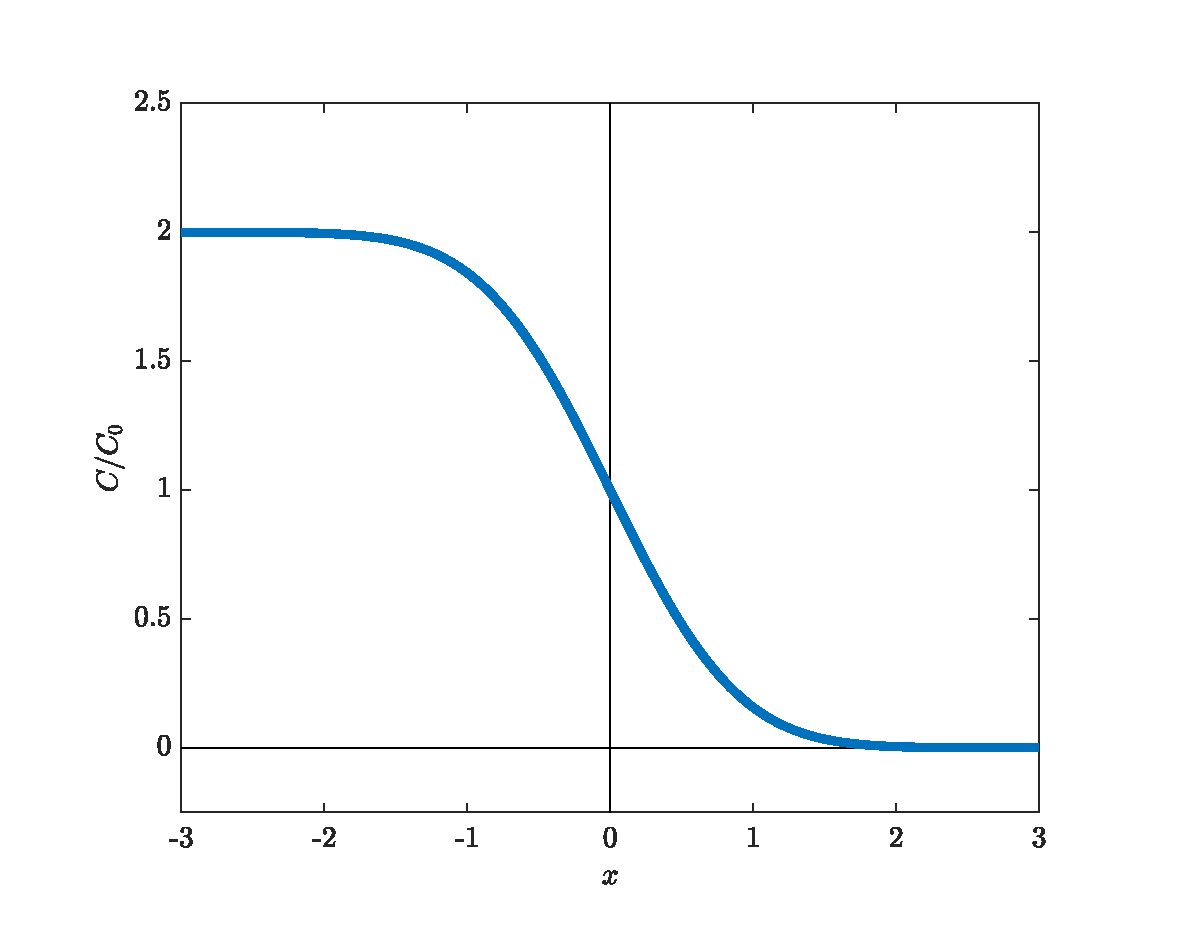
\includegraphics[width = \textwidth]{chapter_2/plot_erfc.pdf}
    \vspace*{-40pt}
    \caption[]{Plot of the complementary error function.}
    \label{fig:plot_erfc}
\end{figure}

The concentration at the source ($x = 0$) is $C_0$, in accordance with the boundary condition, decreases linearly for the region near the interface, and is followed by an exponential decay that goes to zero when we are too far from the source.
